\section{Random Matrix Filtering}
\label{sec:rmt}

This section asks which parts of the empirical correlation matrix are compatible with the RMT sampling-noise benchmark and which are candidates for collective structure. We report the eigenspectrum, reconstruct interpretable components and use robustness checks to delimit the economic reading of the modes. The results describe full-sample structure; they do not estimate time-varying factors.

\subsection{Empirical eigenspectrum}

Random Matrix Theory supplies the spectral benchmark for distinguishing structured collective modes from sampling noise in the empirical correlation matrix \cite{laloux_1999_noise,plerou_2002_random}. The core historical matrix uses $N=58$ assets and $T=1527$ observations, giving $Q=T/N\approx26.33$. The Mar\v{c}enko--Pastur bounds are $\lambda_-=0.6482$ and $\lambda_+=1.4278$.

\begin{center}
\captionof{table}{RMT summary for the core historical universe.}
\label{tab:rmt_summary}
\resizebox{\linewidth}{!}{%
\begin{tabular}{rrrrrrrrrrr}
\toprule
$N$ & $T$ & $Q$ & $\lambda_-$ & $\lambda_+$ & $\lambda_1$ & $\lambda_2$ & $\lambda_3$ & $\lambda_4$ & $\lambda_5$ & Above $\lambda_+$ \\
\midrule
58 & 1527 & 26.33 & 0.6482 & 1.4278 & 21.6505 & 3.0957 & 1.7839 & 1.6543 & 1.4835 & 5 \\
\bottomrule
\end{tabular}}
\end{center}
\GlobalPrecisionNote

Table~\ref{tab:rmt_summary} reports the numerical inputs for RMT filtering. With $N=58$ assets and $T=1527$ complete observations, the aspect ratio is $Q=26.33$, which implies a relatively narrow Mar\v{c}enko--Pastur noise band from $\lambda_-=0.6482$ to $\lambda_+=1.4278$. The first eigenvalue, $\lambda_1=21.6505$, is therefore not a marginal deviation from the random-matrix benchmark but a dominant collective component. The next four eigenvalues, $\lambda_2=3.0957$, $\lambda_3=1.7839$, $\lambda_4=1.6543$ and $\lambda_5=1.4835$, also exceed the upper random bound. There are 5 sample eigenvalues outside the band: these are the candidate collective modes, indicating one broad market mode and four additional modes that may be associated with group, sectoral or localized dependency structure.

Figure~\ref{fig:rmt_spectrum} shows the spectrum against the random benchmark. The largest eigenvalue lies far above the Mar\v{c}enko--Pastur upper bound. Four additional eigenvalues also exceed the upper edge, indicating a dominant market mode and a small number of group or sector modes.

\begin{center}
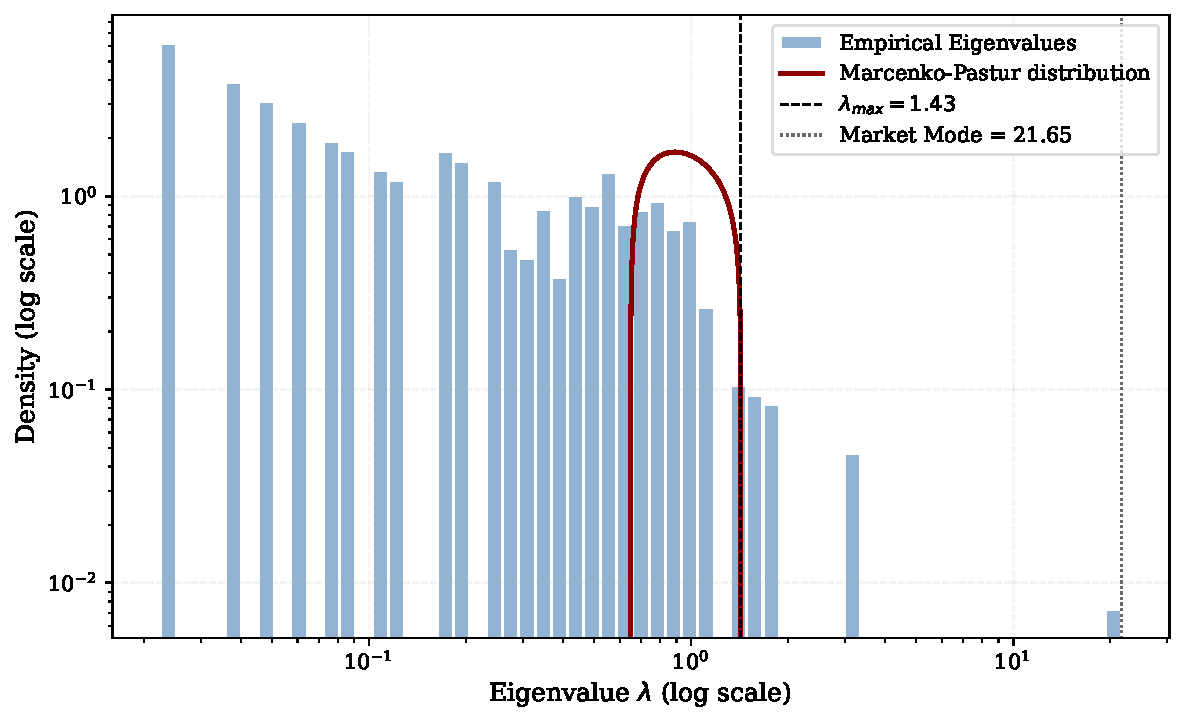
\includegraphics[width=0.80\linewidth]{images/figure_6_rmt_eigenvalue_spectrum.pdf}
\captionof{figure}{Empirical eigenvalue spectrum and Mar\v{c}enko--Pastur bounds. The largest eigenvalue is far outside the random band and captures the market-mode component.}
\label{fig:rmt_spectrum}
\end{center}


\subsection{Market Mode and significant eigenvalues}

The largest eigenvalue is 21.6505, corresponding to approximately 37.3\% of the total trace of the correlation matrix. Its eigenvector has broadly positive loadings, confirming its interpretation as a market mode. It captures broad co-movement and explains why the original correlation matrix has a strong positive common component. The next four eigenvalues are 3.0957, 1.7839, 1.6543 and 1.4835. These values are above $\lambda_+$ and act as candidates for group or sector structure.

The market mode is meaningful but visually dominant. If a network is built directly from the original matrix, many edges can reflect market-wide co-movement instead of local structure. We construct the group-mode matrix to ask what remains after the broad common component is removed.


\subsection{Matrix reconstruction}

The reconstruction step checks that the spectral decomposition and the filtered matrices are being computed accurately. If all eigenvalue--eigenvector modes are recombined, the original correlation matrix is recovered up to floating-point precision. Table~\ref{tab:rmt_reconstruction} reports this numerical check: the Frobenius reconstruction error is approximately $2.74\times10^{-14}$, and the maximum absolute reconstruction error is approximately $3.99\times10^{-15}$. The reported unit diagonal refers to the filtered matrix after the partial reconstruction has been rescaled for downstream correlation-based distances. This check reduces the possibility that subsequent network differences are driven by numerical reconstruction error rather than by the intended selection of market, group and noise-compatible modes.

\begin{center}
\captionof{table}{RMT reconstruction diagnostics.}
\label{tab:rmt_reconstruction}
\begin{tabular}{lr}
\toprule
Diagnostic & Value \\
\midrule
Frobenius reconstruction error & $2.74\times10^{-14}$ \\
Maximum absolute reconstruction error & $3.99\times10^{-15}$ \\
$C_{\mathrm{filtered}}$ diagonal min & 1.0000 \\
$C_{\mathrm{filtered}}$ diagonal max & 1.0000 \\
Eigenvalues above $\lambda_+$ & 5 \\
Market-mode trace share & 0.3733 \\
\bottomrule
\end{tabular}
\end{center}
\GlobalPrecisionNote

Figure~\ref{fig:rmt_filtered_matrices} contrasts the original correlation matrix with the candidate group/sector component. This focused comparison makes the effect of market-mode removal readable in the main text. The market, noise-compatible and retained components are reported in the supplementary full decomposition.

Empirically, the eigenvectors beyond the leading component show loading patterns suggesting localized or sector-related dependencies. This residual organization motivates the clustering and network sections: if localized dependency patterns remain after market-mode removal, MST and PMFG structures should differ when constructed from the group-mode matrix.

\begin{center}
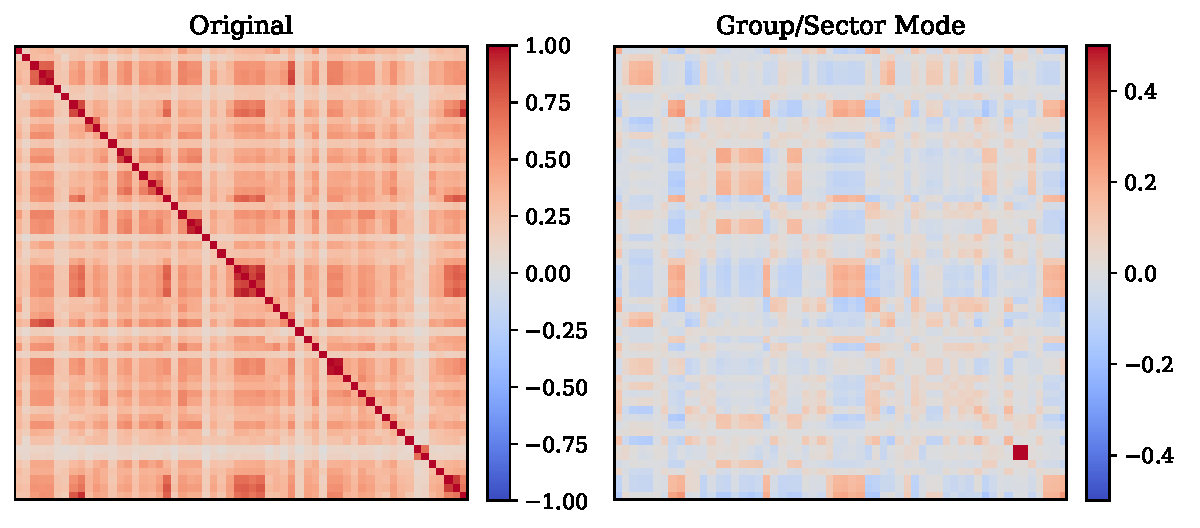
\includegraphics[width=\linewidth]{images/figure_8_original_group_matrices.pdf}
\captionof{figure}{Original and candidate group/sector RMT components at readable scale. The original matrix is dominated by broad positive co-movement, whereas the group/sector component highlights weaker localized contrasts after the leading market mode is removed.}
\label{fig:rmt_filtered_matrices}
\end{center}

\clearpage

\subsection{Top eigenvector loadings}

Eigenvalues identify the strength of collective modes, but eigenvectors help interpret their composition. Figure~\ref{fig:eigenvector_loadings} reports the largest loadings for the five modes above the Mar\v{c}enko--Pastur upper bound. For each eigenvector, assets are ranked by the magnitude of their loadings. The signs of eigenvector loadings are arbitrary up to multiplication by $-1$; the relevant information is therefore the relative contrast between groups of assets, together with the magnitude and concentration of their loadings.

The first eigenvector is a broad market mode. All 58 assets have positive loadings, ranging from 0.037 to 0.174, and the leading mode accounts for 37.3\% of the trace of the correlation matrix. The largest loadings include steel, mining and financial assets, but the positive contribution is distributed across all sectors. This pattern supports its interpretation as market-wide co-movement rather than a sector-specific factor.

The second eigenvector ($\lambda_2=3.10$) is best read as a relative contrast between mining and steel firms---including VALE3, BRAP3/4, GGBR3/4, GOAU3/4, CSNA3 and USIM3/5---and a group led by utilities and selected consumer-cyclical assets. It therefore contains a commodity-related dimension, but it is not a pure Basic Materials factor. The third eigenvector ($\lambda_3=1.78$) similarly contrasts the financial pole formed by BBDC3/4, ITSA4 and BBAS3 with a more heterogeneous industrial, chemical and consumer-cyclical pole led by ROMI3, SHUL4, BRKM3, ALPA4 and GUAR3.

The fourth eigenvector ($\lambda_4=1.65$) is highly concentrated in TELB3 and TELB4, the two listed TELEBRAS share classes. We interpret this result as an issuer-specific share-class component, rather than as evidence of a broad telecommunications factor. The fifth eigenvector ($\lambda_5=1.48$) separates a coherent utilities block---including CEMIG, COPEL, Eletrobras, CPFL Energia and ISA CTEEP---from financial and selected consumer-cyclical assets. This is a plausible utilities-related pattern, but $\lambda_5$ lies only about 3.7\% above the Mar\v{c}enko--Pastur upper bound. Its economic interpretation should therefore remain cautious and be treated as a candidate localized mode.

Overall, Figure~\ref{fig:eigenvector_loadings} shows that the modes beyond the market component are structured contrasts, rather than one-sector classifications. They can mix sectors when firms share macroeconomic, liquidity or balance-sheet exposures. This interpretation motivates the subsequent clustering and network analyses, which test whether these spectral contrasts reappear in other representations of the dependency matrix.

\subsection{Issuer-level share-class robustness}

The 58-asset panel contains 12 companies represented by two listed share classes. This can amplify issuer-specific co-movement and, in the case of TELEBRAS, produces a component that is not an economically broad sector factor. We therefore repeat the RMT calculation after retaining one deterministic representative per company, reducing the panel to 46 issuers. The retained series is the class with the most valid daily returns in the raw historical file, with alphabetical tie-breaking; this rule is stated in Section~\ref{sec:methodology}.

\begin{center}
\captionof{table}{Issuer-level RMT robustness check. The collapsed panel retains one share class per company.}
\label{tab:issuer_rmt_robustness}
\begin{tabular}{lrrrrrr}
\toprule
Panel & $N$ & $T$ & $Q$ & $\lambda_+$ & Modes above $\lambda_+$ & $\lambda_1/N$ \\
\midrule
Full share-class panel & 58 & 1527 & 26.33 & 1.4278 & 5 & 0.3733 \\
Issuer-collapsed panel & 46 & 2207 & 47.98 & 1.3096 & 3 & 0.3363 \\
\bottomrule
\end{tabular}
\end{center}
\GlobalPrecisionNote

The dominant market component is robust: its trace share remains 33.6\% after issuer collapse, compared with 37.3\% in the full panel. Three eigenvalues remain above the issuer-panel bound, so the market mode and two additional collective components are not artifacts of duplicated share classes. In contrast, the TELEBRAS share-class component necessarily disappears, and the two weaker full-panel modes do not remain above the issuer-panel comparison. The principal market-structure result is therefore robust, whereas interpretations of marginal localized modes should account for issuer representation.

\clearpage

\begin{center}

\includegraphics[width=\linewidth]{images/figure_7b_rmt_top_eigenvectors_top_loadings.pdf}
\captionof{figure}{Top eigenvector loadings for the five RMT modes above the Mar\v{c}enko--Pastur upper bound. Eigenvector 1 is a broad market mode. Subsequent eigenvectors show relative contrasts between groups of assets; their overall signs are arbitrary.}
\label{fig:eigenvector_loadings}
\end{center}

\subsection{Circular-shift null robustness}

The Mar\v{c}enko--Pastur benchmark assumes an idealized independent-noise setting. As a complementary check, we compare the five leading eigenvalues with 1,000 independent circular-shift surrogates. Each surrogate preserves the temporal ordering and marginal distribution of every individual return series while breaking their same-date alignment. Table~\ref{tab:rmt_circular_shift_null} reports rank-specific 95th-percentile thresholds and Monte Carlo exceedance probabilities.

\begin{center}
\captionof{table}{Circular-shift null check for the five leading eigenvalues. The null uses 1,000 independent circular shifts, one per asset and replicate.}
\label{tab:rmt_circular_shift_null}
\begin{tabular}{rrrr}
\toprule
Rank & Empirical $\lambda$ & Null 95th percentile & Monte Carlo $p$ \\
\midrule
1 & 21.6505 & 1.6882 & $<0.001$ \\
2 & 3.0957 & 1.4932 & $<0.001$ \\
3 & 1.7839 & 1.3889 & $<0.001$ \\
4 & 1.6543 & 1.3533 & $<0.001$ \\
5 & 1.4835 & 1.3295 & $<0.001$ \\
\bottomrule
\end{tabular}
\end{center}
\GlobalPrecisionNote

All five empirical eigenvalues exceed the rank-matched 95th-percentile circular-shift threshold, including the fifth mode. Thus, its departure from the noise bulk is not explained solely by the temporal dependence or non-Gaussian marginal behavior retained by this surrogate null. This result should be read jointly with the issuer-collapsed check: the fifth mode is statistically distinguishable from this synchronization-free null, but its detailed economic interpretation remains sensitive to how multiple share classes are represented.
